\documentclass{beamer}

\mode<presentation>
{
  \usetheme{default}
  \usecolortheme{default}
  \usefonttheme{default}
  \setbeamertemplate{navigation symbols}{}
  \setbeamertemplate{caption}[numbered]
} 

\usepackage[english]{babel}
\usepackage[utf8x]{inputenc}

\title{Terminverwaltung App Projekt}
\author{Programmierung Java 2}
\date{21. Mai 2019}

\begin{document}

\begin{frame}
  \titlepage
\end{frame}

%\begin{frame}{Outline}
%  \tableofcontents
%\end{frame}

\section{Ziel}

\begin{frame}{Ziel}

\begin{itemize}
  \item REST API Server als Backend für eine Web App
  \item Terminmanagement und Patientenverwaltung 
\end{itemize}

\vskip 1cm

\begin{block}{Web App}
Angular Projekt für Webaufbau - SS19
\end{block}

\end{frame}

\section{Architektur}

\subsection{Web Server}

\begin{frame}{Web Server}

\begin{itemize}
\item Spring Boot
\item Spring Framework + Embedded HTTP(s) Servers - XML Configuration oder @Configuration
\item Ökosystem von Spring (Spring ORM, Spring Security, ...)
\end{itemize}

\end{frame}


\begin{frame}{Web Server}

\begin{itemize}
\item Tomcat als HTTP(s) Server
\item Endpoints (Pfade):
   \begin{itemize}
     \item /api/\{model\} \hspace{10mm} (GET/POST)
     \item /api/\{model\}/\{id\} \hspace{2mm} (PUT/DELETE)
   \end{itemize}
\item Request Type: "application/x-www-form-urlencoded"
\item Response Type: "application/json"
\item Authorization: Basic Auth
\end{itemize}

\end{frame}


\subsection{Datenbank und ORM}

\begin{frame}{Datenbank}

\begin{itemize}
\item MySQL als Datenbank
   \begin{itemize}
     \item MySQL Connector
   \end{itemize}
\item Spring Data JPA als ORM
   \begin{itemize}
     \item Hibernate/JPA
     \item Entity, Repository, ...
   \end{itemize}
\end{itemize}

\end{frame}

\subsection{Modelle}


\begin{frame}{Modelle}

\begin{itemize}
\item User
\item Patient
\item Address
\item Appointment
\item AppointmentRecord
\item Prescription
\item Medicine
\item Disease
\end{itemize}

\end{frame}


\subsection{Beispiel}

\begin{frame}{Beispiel}

\begin{figure}
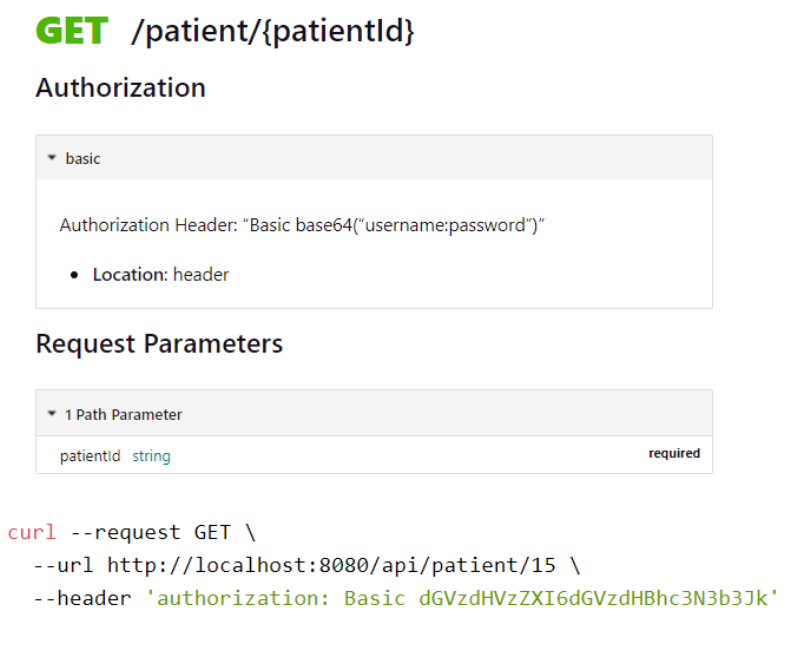
\includegraphics[width=95mm]{GET.png}
\end{figure}

\end{frame}

\begin{frame}

\begin{figure}
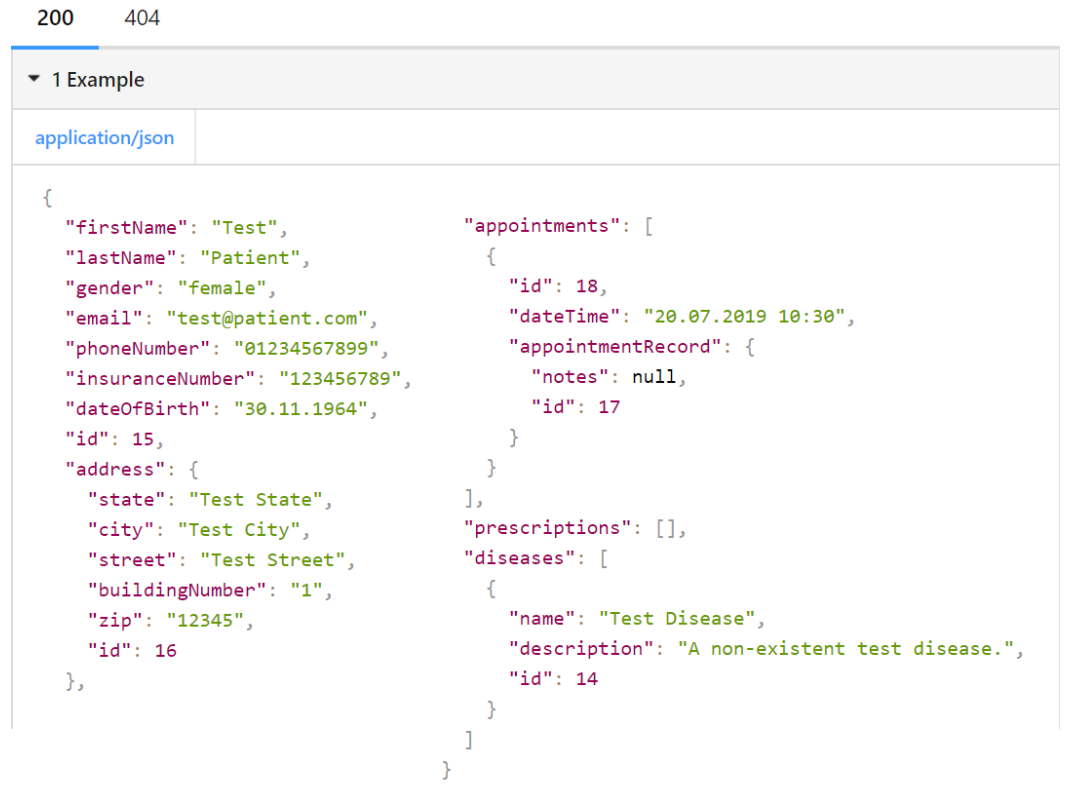
\includegraphics[width=105mm]{GET_RES.png}
\end{figure}

\end{frame}


\begin{frame}

\begin{figure}
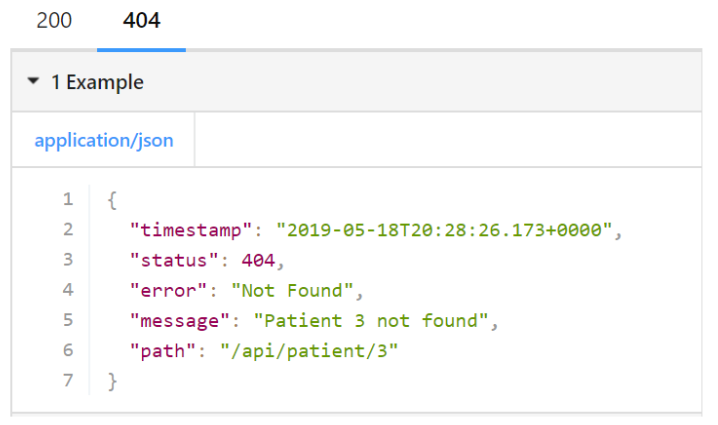
\includegraphics[width=90mm]{GET_404.png}
\end{figure}

\end{frame}

\begin{frame}{TODO}

\begin{itemize}
\item Effizientere Datenabfragen (Extra Pfade mit Filtern)
\item Validierung (Hibernate Validator statt MySQL Fehler)
\item Komplette API-Dokumentation (Swagger - OpenAPIv2)
\end{itemize}

\end{frame}

\end{document}
